\chapter{Theory}

\section{Standard Model}
-current status of SM. quick overview

\section{Non-resonant new Physics}
- BSM physics
- non-resonance

\newpage
\subsection{Contact Interaction Theory}
%\addcontentsline{toc}{section}{Contact Interaction Theory}

- more history is needed here\\

Contact interactions (CI) can be used to describe a variety of Beyond the Standard Model phenomena such as quark/lepton compositness. (describe quark-lepton compositness). At ATLAS contact interactions are being searched for as a 4-fermion contact interaction between two quarks from the incoming protons and two final state leptons.

\begin{figure}[h]
\begin{center}
   %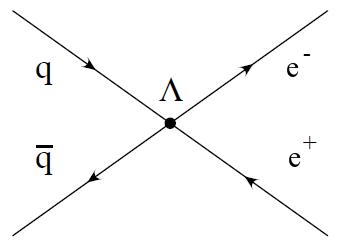
\includegraphics[scale=0.3]{images/fd2.png}
   %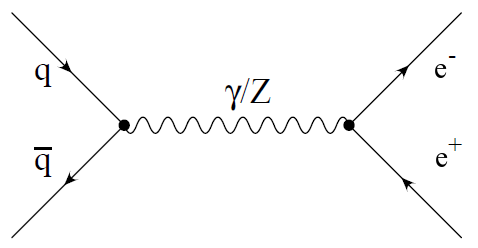
\includegraphics[scale=0.4]{images/fd1.png}
\end{center}
\caption{Feynman diagrams of a contact interaction (left) and the predominant background Drell-Yan production (right).}
\label{fig:fd}
\end{figure}

Experimentally this interaction would be seen as a deviation from the Standard Model (SM) Drell-Yan (DY)($q\bar{q}~\rightarrow~\gamma/Z~\rightarrow~\ell^{+}\ell^{-}$) dilepton mass spectrum (seen in Fig. \ref{fig:fd}). 

Without knowing the intermediate process one can write a Lagrangian describing the new Interaction:
\begin{equation}
        \mathcal{L} = \frac{g^{2}}{2\Lambda^{2}}
                [\eta_{LL} (\bar{\psi_{L}}\gamma_{\mu}\psi_{L}) (\bar{\psi_{L}}\gamma^{\mu}\psi_{L}) 
                + \eta_{RR} (\bar{\psi_{R}}\gamma_{\mu}\psi_{R}) (\bar{\psi_{R}}\gamma^{\mu}\psi_{R}) 
                + 2\eta_{LR} (\bar{\psi_{L}}\gamma_{\mu}\psi_{L}) (\bar{\psi_{R}}\gamma^{\mu}\psi_{R}) ].
\end{equation}
The sign of $\eta$ defines whether the new interaction interferes constructively ($\eta = -1$) or destructively ($\eta = +1$) with the DY background interaction. For previous analyses \cite{CDF, D0, ATLAS} a benchmark model of just the Left-Left (LL) component has been used and defined by $\eta_{LL} = \pm~1$ and $\eta_{RR} = \eta_{LR} = 0$. Here however an investigation of each of the three parameters is done individually. Both the LL and RR cases are expected to behave similarly however the LR case exhibits a different angular dependence than either of the other formalisms or the DY background.
A differential cross section for this new interaction is given by
\begin{equation}
        \frac{d\sigma}{dm_{\ell\ell}} = 
                \frac{d\sigma_{DY}}{dm_{\ell\ell}} 
                - \eta\frac{F_{I}}{\Lambda^{2}} 
                + \frac{F_{C}}{\Lambda^{4}},
\label{eq:DiffCross}
\end{equation}
where $m_{\ell\ell}$ is the dilepton mass and $\Lambda$ is the scale of the new physics. In the case of quark/lepton compositness $\Lambda$ refers to the point at which fermions stop being bound as SM quarks and leptons. $F_{I}$ and $F_{C}$ define the interference DY-CI term and the pure CI term respectively. The experimental signature of this effect is a broad increase on the SM background at high invariant mass for all models while the LR formalism also sees a different forward backwards asymmetry.


\newpage





\subsection{ADD Theory}
%\addcontentsline{toc}{section}{ADD Theory}
ADD is a theory used to solve the hierarchy problem via large extra spacial dimensions first described by Arkani-Hamed, Dimopoulos, and Dvali (ADD) \cite{ADD}. The ADD model predicts a graviton that propagates the extra dimensions and acquires Kaluza-Klein (KK) modes that show as a broad increase in the SM background. This is the reason the search for ADD is done in conjunction with CI.


